\documentclass{article}

\usepackage{fullpage}
\usepackage{amsmath}
\usepackage{amssymb}
\usepackage{bm}
\usepackage{multicol}
\usepackage{graphicx}
\usepackage{float}
\usepackage{framed}
\usepackage{xcolor}

\usepackage{tensor}

\usepackage[backend=bibtex, sorting=nyt, style=alphabetic]{biblatex}
\addbibresource{main.bib}

\newcommand{\parHeading}[1]{\underline{\textbf{#1}}}
\newcommand{\doubleline}{\\[2\baselineskip]}

\begin{document}

\title{\fontfamily{lmr} \Huge  Analysis of Particle Kinetics in Curved Space-time}

\author{\Large Olaf Willocx, Lars Meulenijzer, Areen Raj}
\date{2026}

\maketitle

\begin{center} 
\vspace{-15pt} 
\Large \textit{Selected Topics in Mathematics II\textnormal{ (G0L86A), KU Leuven}}
\end{center}


\thispagestyle{empty}
\vspace{40pt}


\section*{Introduction}

Investigating the behavior of particles in a background of curved spacetime requires being able to model their geodesics. For some known curved spacetime metrics, like the Schwarzschild metric and the Kerr metric, analytical orbits are known. However, most particle trajectories cannot be known analytically and have to be solved numerically. A scenario where this is needed is the modeling of plasmas near a black hole using kinetic codes like particle-in-cell (PIC). A common numerical framework for solving particle orbits in general relativity (GR) involves splitting the metric into spatial slices parameterized by time. This formalism is called the Arnowitt-Deser-Misner (ADM) formalism. Using this formalism, we implement an integration scheme that explicitly conserves the energy of the particle \cite{Bacchini_2018}\cite{Bacchini_2019} while solving its orbit. To run PIC simulations in GR, it is also necessary to solve the Maxwell equations in curved spacetime. We don't implement the full Vlasov-Maxwell, but instead limit ourselves to the Vlasov-Poisson system in which charges are approximated as static. We then apply the implemented method to the two-stream instability in the presence of a black hole.\\
\\
In section ..., we introduce the equations that are needed for solving geodesics in the ADM formalism. In section ..., we discuss the Maxwell equations in curved spacetime and give an analytical solution. In section ..., we discuss how curved spacetime affects the dynamics of plasma. This knowledge is then applied to the two-stream instability. In section ..., we discuss orbits around Schwarzschild and Kerr black holes for which analytic formulae exist. In section ..., we explain the integration scheme that is used for evolving particles along their geodesics. In section ..., we give an overview of the algorithm that is used for simulating particles with the Vlasov-Poisson system in curved spacetime, for one-dimensional simulations. In section ..., the results of our simulations are shown and discussed.

\section{Geodesics in the ADM formalism}

Any spacetime metric $g_{\mu\nu}$ can be rewritten as \cite{rezzolla2013}
\begin{equation}
    g_{\mu\nu} = 
    \begin{pmatrix}
    -\alpha^2+\beta_k\gamma^{kl}\beta_l & \beta_i\\
    \beta_j & \gamma_{ij}
    \end{pmatrix}.
\end{equation}
Here $\alpha$ is the lapse function, $\beta_i$ is the shift vector, and $\gamma_{ij}$ is the spatial metric. We use the (-,+,+,+) metric convention, as well as $c=1$ for the speed of light. The decomposition is also referred to as the 3+1 split of the metric. The coordinate time $t \equiv x^0$ parameterizes 3D slices of space that have a metric $\gamma_{ij}(t)$. These slices are spacelike hypersurfaces $\Sigma_t$ on which the time coordinate $t$ is constant. The ADM formalism allows for particles and fields to live on the 3D slices of foliated space. The evolution of the particles and fields can then be parameterized by $t$. Computationally, this makes it much easier to model particle trajectories than using a 4D approach. Both massless and massive particles follow geodesics, which are constrained by the set of four equations
\begin{equation}
    \frac{\text{d}^2x^\rho}{\text{d}\tau^2} + \Gamma^\rho_{\mu\nu} \frac{\text{d}x^\mu}{\text{d}\tau} \frac{\text{d}x^\nu}{\text{d}\tau} = 0.
\end{equation}
Here $\tau$ is the proper time along the geodesic and $\Gamma^\rho_{\mu\nu}$ are the Christoffel symbols. The contravariant four-velocity of the particle is defined as $u^\mu \equiv \frac{\text{d}x^\mu}{\text{d}\tau}$. From the definition of the proper time along the geodesic, it can be shown that $u^0$ is constrained by the relation
\begin{equation}
    u^0 = \frac{\sqrt{\epsilon + u_i\gamma^{ij}u_j}}{\alpha}
\end{equation}
where $\epsilon = 0$ for massless particles and $\epsilon = 1$ for massive particles. This equation can also be rewritten as $u^\mu u_\mu = -\epsilon$, showing that the norm of the four-velocity $u_\mu$ is conserved. The definition of the four-velocity can be rewritten to get an equation for evolving the particle's position:
\begin{equation}
    \frac{\text{d}x^i}{\text{d}t} = \gamma^{ij}\frac{u_j}{u^0} - \beta^i.
\end{equation}
The geodesic equation can be rewritten and expanded using the ADM formalism, resulting in an equation for evolving the particle's momentum:
\begin{equation}
    \frac{\text{d}u_i}{\text{d}t} = -\alpha u^0\partial_i\alpha + u_j\partial_i\beta^j - \frac{u_ju_k}{2u^0}\partial_i\gamma^{jk}.
\end{equation}
Given initial conditions $x^i$ and $u_i$, the last three equations are sufficient to be able to evolve both massive and massless particles through the spacetime with metric $g_{\mu\nu}$.


\section{Maxwell equations in curved spacetime}

The electric and magnetic fields are 3-vectors that live on the spacelike hypersurfaces $\Sigma_t$. However, these fields can also be seen as 4-vectors that are tangent to $\Sigma_t$ \cite{Alcubierre2009}. The 4-vector $n_\mu = (-\alpha, 0, 0, 0)$ is a unit vector that is perpendicular to $\Sigma_t$ \cite{Alcubierre2009} and that satisfies the relation $n_\mu n^\mu = -1$. The electric and magnetic fields $E^\mu$ and $B^\mu$, written as 4-vectors, must be perpendicular to $n_\mu$. Therefore, the zeroth components $E^0$ and $B^0$ must be zero. A projection operator that projects 4-vectors onto $\Sigma_t$ can be defined as
\begin{equation}
    {h_\mu}^\nu \equiv {\delta_\mu}^\nu + n_\mu n^\nu.
\end{equation}
With this projection operator, the Maxwell equations can be written in the language of the ADM formalism. Let $j^\mu$ be the four-current, with $\rho \equiv -n_\mu j^ \mu$ the charge. The Maxwell equations then are
\cite{Alcubierre2009}
\begin{equation}
\begin{aligned}
    &{h_\mu}^\nu \nabla_\nu E^\mu = 4\pi\rho\\
    &{h_\mu}^\nu \nabla_\nu B^\mu = 0\\
    &\alpha {h^i}_\nu (n^\rho \partial_\rho E^\nu - E^\rho \partial_\rho n^\nu) = \epsilon^{ijk} \partial_j (\alpha B_k) + \alpha K E^i - 4\pi\alpha {h^i}_\mu j^\mu\\
    &\alpha {h^i}_\nu (n^\rho \partial_\rho B^\nu - B^\rho \partial_\rho n^\nu) = -\epsilon^{ijk} \partial_j (\alpha E_k) + \alpha K B^i
\end{aligned}
\end{equation}
where $K \equiv -\nabla_\mu n^\mu$ is the trace of the extrinsic curvature of $\Sigma_t$. As an example, we set $j^\mu = 0$ and use the above equations to derive an analytic solution in a scenario with a relatively simple spacetime metric.

\subsection{An analytic solution}

This subsection considers a simple curved metric for which an analytic wave solution of the Maxwell equations can be found. The spacetime metric that is considered is the static metric of the Newtonian gauge
\begin{equation}
    g_{\mu\nu} = \begin{pmatrix}
        -(1+2\Phi) & 0 & 0 & 0\\
        0 & 1-2\Phi & 0 & 0\\
        0 & 0 & 1-2\Phi & 0\\
        0 & 0 & 0 & 1-2\Phi
    \end{pmatrix}
\end{equation}
with $\Phi(x^\mu)$ a scalar function. This metric is a solution of the linearized Einstein field equations in the absence of anisotropic pressure \cite{1995ApJ}. In other words, as long as the scalar $|\Phi|$ is much smaller than $1$, this metric is an approximate solution of the Einstein field equations. In the presence of anisotropic pressure, the metric is parameterized by two scalars instead of only $\Phi$. The scalar $\Phi$ can be interpreted as the gravitational potential \cite{1995ApJ}. Because the metric is diagonal, the trace of the extrinsic curvature vanishes ($K = 0$), and the spatial part of the projection operator is ${h_i}^j = {\delta_i}^j$. The Maxwell equations thus simplify:
\begin{equation}
\begin{aligned}
    &\nabla_i E^i = 0 \qquad&&\partial_t E^i = \epsilon^{ijk} \partial_j (\alpha B_k)\\
    &\nabla_i B^i = 0 \qquad&&\partial_t B^i = -\epsilon^{ijk} \partial_j (\alpha E_k).
\end{aligned}
\end{equation}
We consider wave solutions of the electric and magnetic fields using the following ansatz:
\begin{equation}
\begin{aligned}
    &\partial_y \Phi(x) = 0 \qquad&&E^i = \big(0, E_0 e^{i(k(x)x-\omega t)}, 0\big)\\
    &\partial_z \Phi(x) = 0 \qquad&&B^i = \big(0, 0, B_0 e^{i(k(x)x-\omega t)}\big).
\end{aligned}
\end{equation}
The physical interpretation behind this ansatz is that of a photon diving straight into or climbing out of a gravitational well. This ansatz already satisfies two of the Maxwell equations. Filling in this ansatz into the remaining Maxwell equations gives the following constraints:
\begin{equation}
E_0 = B_0 \qquad\text{and}\qquad kx = \omega \int \frac{\text{d}x}{A} + i\log{A} \quad\text{with}\quad A \equiv \sqrt{1 + 2\Phi}(1 - 2\Phi).
\end{equation}
In the limit that spacetime is flat and $\Phi \to 0$, the obtained solutions for the electromagnetic waves become
\begin{equation}
    E^y = E_0 e^{i\omega(x-t)}, \qquad B^z = B_0 e^{i\omega(x-t)}
\end{equation}
which are the familiar solutions we expect to find in flat spacetime. As the waves enter a gravitational well and $\Phi$ becomes negative, $A$ becomes larger than $1$. As a result, two things happen: the amplitude of the wave changes and the wavelength decreases. The decreasing of the wavelength shows that the light is gravitationally blueshifted.\\
\\
As an example, we consider $\Phi = -a \exp{(-x^2/2)}$. $\Phi$ cannot become smaller than $-0.5$, otherwise the metric components change sign. The resulting solution is shown in figure \ref{fig:gravitational_redshift}.

\begin{figure}[ht!]
    \centering
    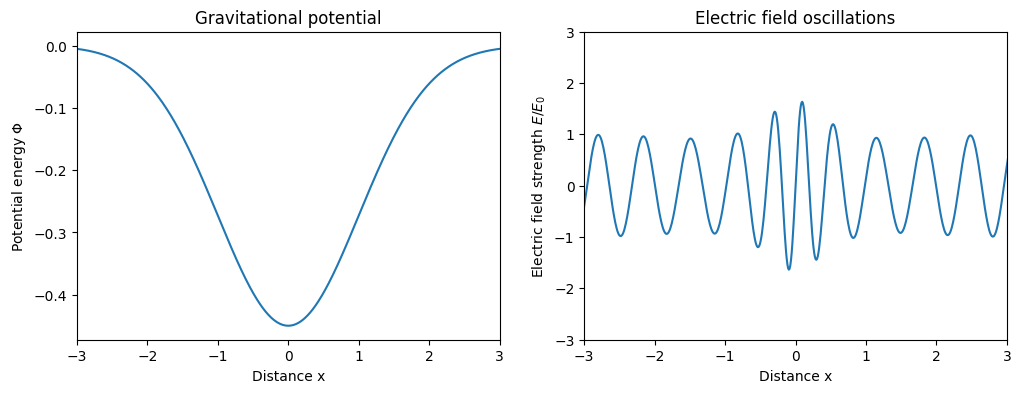
\includegraphics[width=\hsize]{figures/gravitational_redshift.png}
    \caption{The gravitational potential $\Phi = -a \exp{(-x^2/2)}$ with $a = 0.45$ and the corresponding electric field strength at some fixed moment in time. The frequency of the wave is $\omega = 10$ (the units of which are fixed by the units of $x$ and the speed of light).}
    \label{fig:gravitational_redshift}
\end{figure}


\section{Two-stream instability in curved spacetime}

We consider a cold two-stream instability in a diagonal metric, where the streams are moving in the $x_1$-direction with velocities $v_0$ and $-v_0$. At each point, local coordinates $\tilde{t} = \sqrt{-g_{00}} t$ and $\tilde{x}_1 = \sqrt{g_{11}} x_1$ can be chosen so that, in the frame of these local coordinates, spacetime is locally flat. At every point in spacetime, the physics in local coordinates should be the same. In local coordinates, the two-stream instability reduces to the two-stream instability from special relativity. From the perspective of an observer at infinity, the speed of the flow of time at the point $x_\mu$ is altered by a factor $\sqrt{-g_{00}(x_\mu)}$. This effect is gravitational time dilation, and it alters the speed at which instabilities in the two-stream instability grow. We consider the case of a Schwarzschild black hole, for which $\sqrt{-g_{00}} = \sqrt{1 - 2GM/r}$. The closer to the black hole we look, the slower the two-stream instability grows. We assume that the length scale at which the two-stream instability occurs is much smaller than the length scale on which the spacetime metric changes.\\
\\
In the local coordinates, the instability occurs at wave numbers $\tilde{k} = k / \sqrt{g_{11}}$ for which $\tilde{k}^2\tilde{v}_0^2\tilde\gamma_0^3 < \tilde\omega_{p,0}^2$. Here $\tilde{v}_0 = v_0 \sqrt{g_{11}/g_{00}}$ is the speed of the streams in local coordinates, $\tilde\gamma_0 \equiv \gamma(\tilde{v}_0)$ is the corresponding Lorentz factor, and $\tilde\omega_{p,0} = \omega_{p,0}\sqrt{g_{00}}$ is the plasma frequency in local coordinates. From this, we can find an expression for the critical wave number $k_\text{crit}$ in global coordinates: $k^2_\text{crit} v_0^2 \tilde{\gamma}_0^3 = \omega_{p,0}^2$. This equation shows that the curved spacetime only alters the critical wave number through the Lorentz factor. The expression for the critical wave number is altered by a factor $\tilde{\gamma}_0^3 / \gamma_0^3 = \sqrt{1 - v_0^2} / \sqrt{1 - \frac{g_{11}}{-g_{00}} v_0^2}$ compared to the case in flat spacetime. In Figure \ref{fig:k_crit_modification}, the modifying factor $\tilde{\gamma}_0^3 / \gamma_0^3$ is plotted for several values of $v_0$. The presence of the black hole increases $k_\text{crit}$, allowing the instability to occur at smaller length scales than it would in flat spacetime. Both going closer to the black hole and having a larger speed $v_0$ cause a decrease in the factor $\tilde{\gamma}_0^3 / \gamma_0^3$. Figure \ref{fig:k_crit_modification} shows that, for every speed $v_0$, there is a radial distance $r$ at which the modification factor reaches zero. Below that distance, the speed $v_0$ becomes nonphysical, because $\tilde{v}_0$ exceeds the speed of light. This is demonstrated in Figure \ref{fig:accessible_region}, which shows the region of phase space that is accessible by massive particles moving on radial trajectories.\\

\begin{figure}[ht!]
\centering
\begin{minipage}{.48\textwidth}
  \centering
  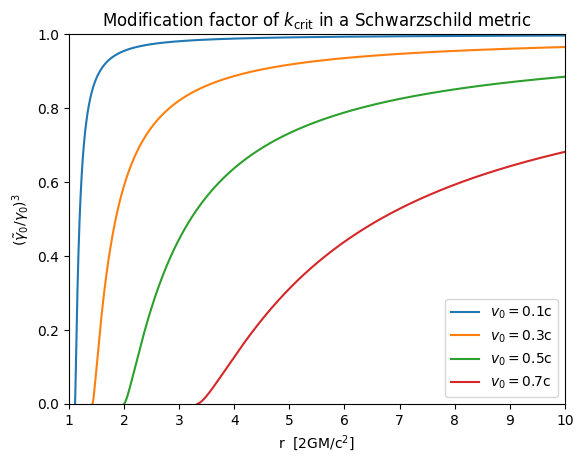
\includegraphics[width=\linewidth]{figures/k_crit_modification.png}
  \caption{The factor $\tilde{\gamma}_0^3 / \gamma_0^3$ near a Schwarzschild black hole as a function of the radial coordinate, for several values of the speed $v_0$.\\\,\\\,}
  \label{fig:k_crit_modification}
\end{minipage}%
\quad
\begin{minipage}{.48\textwidth}
  \centering
  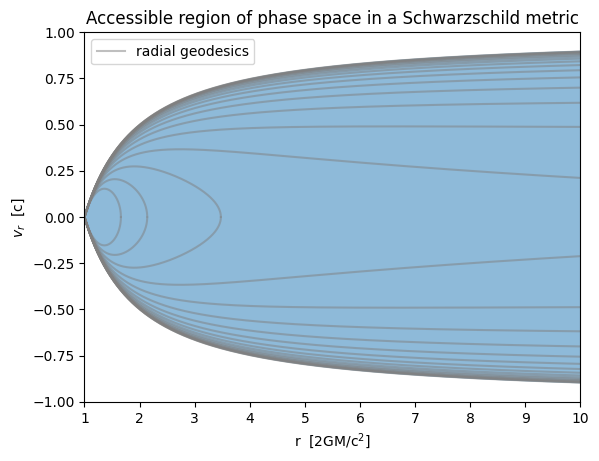
\includegraphics[width=\linewidth]{figures/accessible_region.png}
  \caption{The accessible region of the radial part of phase space near a Schwarzschild black hole, shown as a blue region. The grey curves are geodesics of massive particles moving radially away from and towards the black hole.}
  \label{fig:accessible_region}
\end{minipage}
\end{figure}

\noindent
As the two-stream instability evolves, the gravity of the black hole will cause the speed and density of both streams to change. In general, it will no longer be true that the two streams have the same speed (in absolute values). At each position $x_\mu$, it will still be possible to change to a frame of reference where the streams have speeds $v_0$ and $-v_0$, but in general the densities of the streams will still be different. As a result, the two-stream instability will no longer adhere to the formula $\tilde{k}^2_\text{crit} \tilde{v}_0^2 \tilde{\gamma}_0^3 = \tilde{\omega}_{p,0}^2$.


% olaf: Some brainstorming:

% \section*{Conventions}
% (metric signature)
% (electromagnetic conventions)
% \section*{Geodesics}
% (affine: k_\nu\nabla^\nu k^\mu=0)
% \subsection*{Fermion-electromagnetic deviations}
% (affine: k_\nu\nabla^\nu k^\mu=a_\perp^mu)
% \section*{Particle dynamics in curved spacetimes}
% \subsection*{Kerr spacetimes}
% \subsubsection*{Lightlike orbits}
% \subsubsection*{Timelike orbits}
% \subsubsection*{Timelike magnetically perturbed orbits}
% (In a homogeneous magnetic field?)
% (At the edge of some dipole field from a nearby neutron star?)
% \section*{Geodesic numerics}
% (Relevance of the parameterization?)
% (Will non-affine parameterizations be necessary? Then the theory must be more general.)
% (Coordinate singularity concerns?)
% (Is symplectomorphic integration desirable?)
% (Or exact energy conserving implicit?)
% (Or time-adaptive and not care?)
% \subsection*{Kerr spacetime}
% \subsubsection*{Lightlike orbits}
% (comparison with analytical)
% (render black hole accretion disk or so?)
% \subsubsection*{Timelike orbits}
% (comparison with analytical)
% \subsubsection*{Timelike magnetically perturbed orbits}
% \section*{Electrostatic ${1+1}$ particle-in-cell}
% (numerical details)
% (implementation details)
% \subsection*{$2$-stream instability in Kerr spacetime}
% (Should see electron holes.)
% (What else do we expect, how will it differ?)
% (I suppose this is like an AGN/quasar jet model.)

\section*{Particle Trajectories in Curved Spacetime}
In this section, we will discuss the qualitative nature of the trajectories of both massless and massive particles in the vicinity of black holes. The case under consideration will be that of the Kerr Black Hole, which can be trivially extended to the Schwarzschild solution as well. Our analysis will only cover particles in the region outside the outermost event horizon.

\subsection*{Kerr Spacetime}
First, we once again specify the Kerr metric in the standard Boyer-Lindquist $(t,r,\theta,\phi)$ coordinates. We have taken the gravitational constant and the speed of light both to be unity,

\begin{equation}
    ds^2 = -(1-\frac{2Mr}{\Sigma})dt^2 - \frac{4Mr}{\Sigma}a \sin^2\theta dtd\phi + \Sigma(\frac{dr^2}{\Delta} + d\theta^2) + (r^2 + a^2 + \frac{2Mr}{\Sigma}a^2\sin^2\theta)\sin^2\theta d\phi^2
\end{equation}

where,

\[
    \Sigma = r^2 + a^2\cos^2\theta, \qquad \Delta = r^2 - 2Mr + a^2
\]

and $M$ and $a$ represent the mass and the angular momentum per unit mass of the black hole respectively.\medskip

There are three interesting radial positions to note - two of these are the event horizons that are derived from the roots of $\Delta$ which make the metric singular - ($r_-$ and $r_+$).

The other is the killing horizon where the time Killing vector becomes spacelike - which is the boundary of the ergosphere.
\[
    r_{\pm} = M \pm \sqrt{M^2 - a^2}, \qquad r_{ergo} = M + \sqrt{M^2 - a^2\cos^2\theta}
\]
\\
We will also briefly mention the nomenclature that will be used to classify the trajectories in this report. Namely,

\begin{itemize}
    \item \parHeading{Lightlike vs Timelike}: Lightlike trajectories are those followed by massless particles such as photons, while timelike trajectories are those followed by massive particles. The main difference between the two is that lightlike trajectories have a four-velocity that is null, while timelike trajectories have a four-velocity that is timelike.
    \item \parHeading{Spherical (Circular) vs Non-spherical (Non-circular)}: Spherical trajectories are those that maintain a constant radial coordinate, while non-spherical trajectories are those that do not. When considering only the equatorial plane, these are referred to as circular and non-circular trajectories respectively.
    \item \parHeading{Equatorial vs Non-equatorial}: Equatorial trajectories are those that lie only in the equatorial plane - $\theta = \pi/2$ - while, non-equatorial trajectories are those that do not.
\end{itemize}

Corresponding to this metric, the geodesic equations parameterized by the proper time ($\tau$) are as follows. We have also defined a corollary for the $\theta$ coordinate as $u = \cos\theta$, which represents the latitudinal position of the particle with respect to the black hole.

\begin{subequations} \label{eq:geodesic_equations}
\begin{align}
   \Sigma\frac{dr}{d\tau} = \pm\sqrt{R(r)} \\
   \Sigma\frac{du}{d\tau} = \pm\sqrt{V(u)} \\ 
   \Sigma\frac{d\phi}{d\tau} = \frac{\Phi}{1-u^2} + \frac{a}{\Delta}(2MrE - a\phi) \\
   \Sigma\frac{dt}{d\tau} = -a^2E(1-u^2) + \frac{1}{\Delta}(E(r^2 + a^2)^2 - 2Mra\Phi)
\end{align}
\end{subequations}

where,

\begin{equation} \label{eq:radial_potential}
    R(r) = (E^2 - \mu^2)r^4 + 2M\mu^2r^3 + [a^2(E^2 - \mu^2) - Q - \Phi^2]r^2 + 2M[(aE - \Phi)^2 + Q]r - a^2Q
\end{equation}

\begin{equation} \label{eq:theta_potential}
    V(u) = a^2(\mu^2 - E^2)u^4 - [Q + \Phi^2 + a^2(\mu^2 - E^2)]u^2 + Q
\end{equation}

Here, $\mu$ is the rest mass of the particle. In the case of massive particles we take it to be equal to 1 and in the case of massless particles it is equal to 0. $E$ and $\Phi$ are the energy and the angular momentum of the particle in the direction of rotation of the black hole and $Q$ is the Carter's constant. We will elaborate on the nature of the Carter's constant in the next section, but for now we will just treat it as a constant of motion that is related to the motion of the particle in the $\theta$ direction.

The right hand side of (\ref{eq:geodesic_equations}) represents the total amount of kinetic energy available to the particle - its total energy minus the effective potential it has to overcome.\medskip

We can gain some information about this effective potential by looking at the radial geodesic equation for a specific class of trajectories,
\begin{itemize}
    \item We consider a massless photon moving on null/lightlike geodesics.
    \item The photon starts its motion in the equatorial plane ($\theta = \pi/2$) with zero Carter's Constant.
    \item It is either co-rotating or counter-rotating with respect to the black hole, so $\Phi$ is non-zero.
\end{itemize}

\parHeading{Non-Spherical, Lightlike, Equatorial Motion:} When the RHS of the radial and latitudinal equations ($R(r)$ and $V(u)$) are zero, it represents a turning point where the effective potential is equal to the energy of the particle - causing it to stop. If there is a non-zero force acting on the particle at this point (first derivative of the RHS functions) then it will reverse its motion in that particular direction. \medskip

For the radial case with the conditions that we mentioned above, the RHS reduces to,
\begin{equation}
    \dot{r}^2 = \frac{(r^2+a^2)^2-a^2\Delta}{r^4}(E-V_-)(E-V_+) + \frac{\kappa\Delta}{r^2}
\end{equation}

where,
\begin{equation}
   \boxed{V_{\pm} = \frac{2Mar\Phi \pm r^2|\Phi|\sqrt{\Delta}}{(r^2+a^2)^2-a^2\Delta}}
\end{equation}

$\kappa$ is the constant that leads to the parametrization of the four velocity. In the photon case $\kappa = 0$ since we are considering massless particles.\medskip

The absolute value of $\Phi$ is taken to make sure that $V_+$ is always greater than $V_-$ in the case that the particle is counter-rotating or co-rotating with respect to the black hole.\bigskip

We now state some properties of the effective potentials,

\begin{itemize}
    \item Both the potentials coincide at the outer horizon when $\Delta=0$. This converged potential is positive for co-rotating and negative for counter-rotating photons. Since, we only consider motion outside the outer event horizon for now, therefore, our area of interest starts here. 
    \item At infinity, both the potentials go to zero and they only have one extremum each - which is always a maximum for $V_+$ and a minimum for $V_-$. 
    \item Owing to the presence of the ergosphere, the object can have negative energies in specific regions as we will see. 
\end{itemize}

For allowed ranges of motion the RHS should be non-negative, which can only happen at the following ranges. 

\[ E < V_-, \qquad E > V_+ \]

Any motion outside these two ranges is forbidden since the particle does not have enough energy to overcome the effective potential. Figures \ref{fig:counter_potential_sketch} and \ref{fig:co_potential_sketch} are sketches of the counter-rotating and co-rotating potentials for a specific value of $\Phi$, $M$ and $a$.

\begin{figure}[H]     
    \centering
    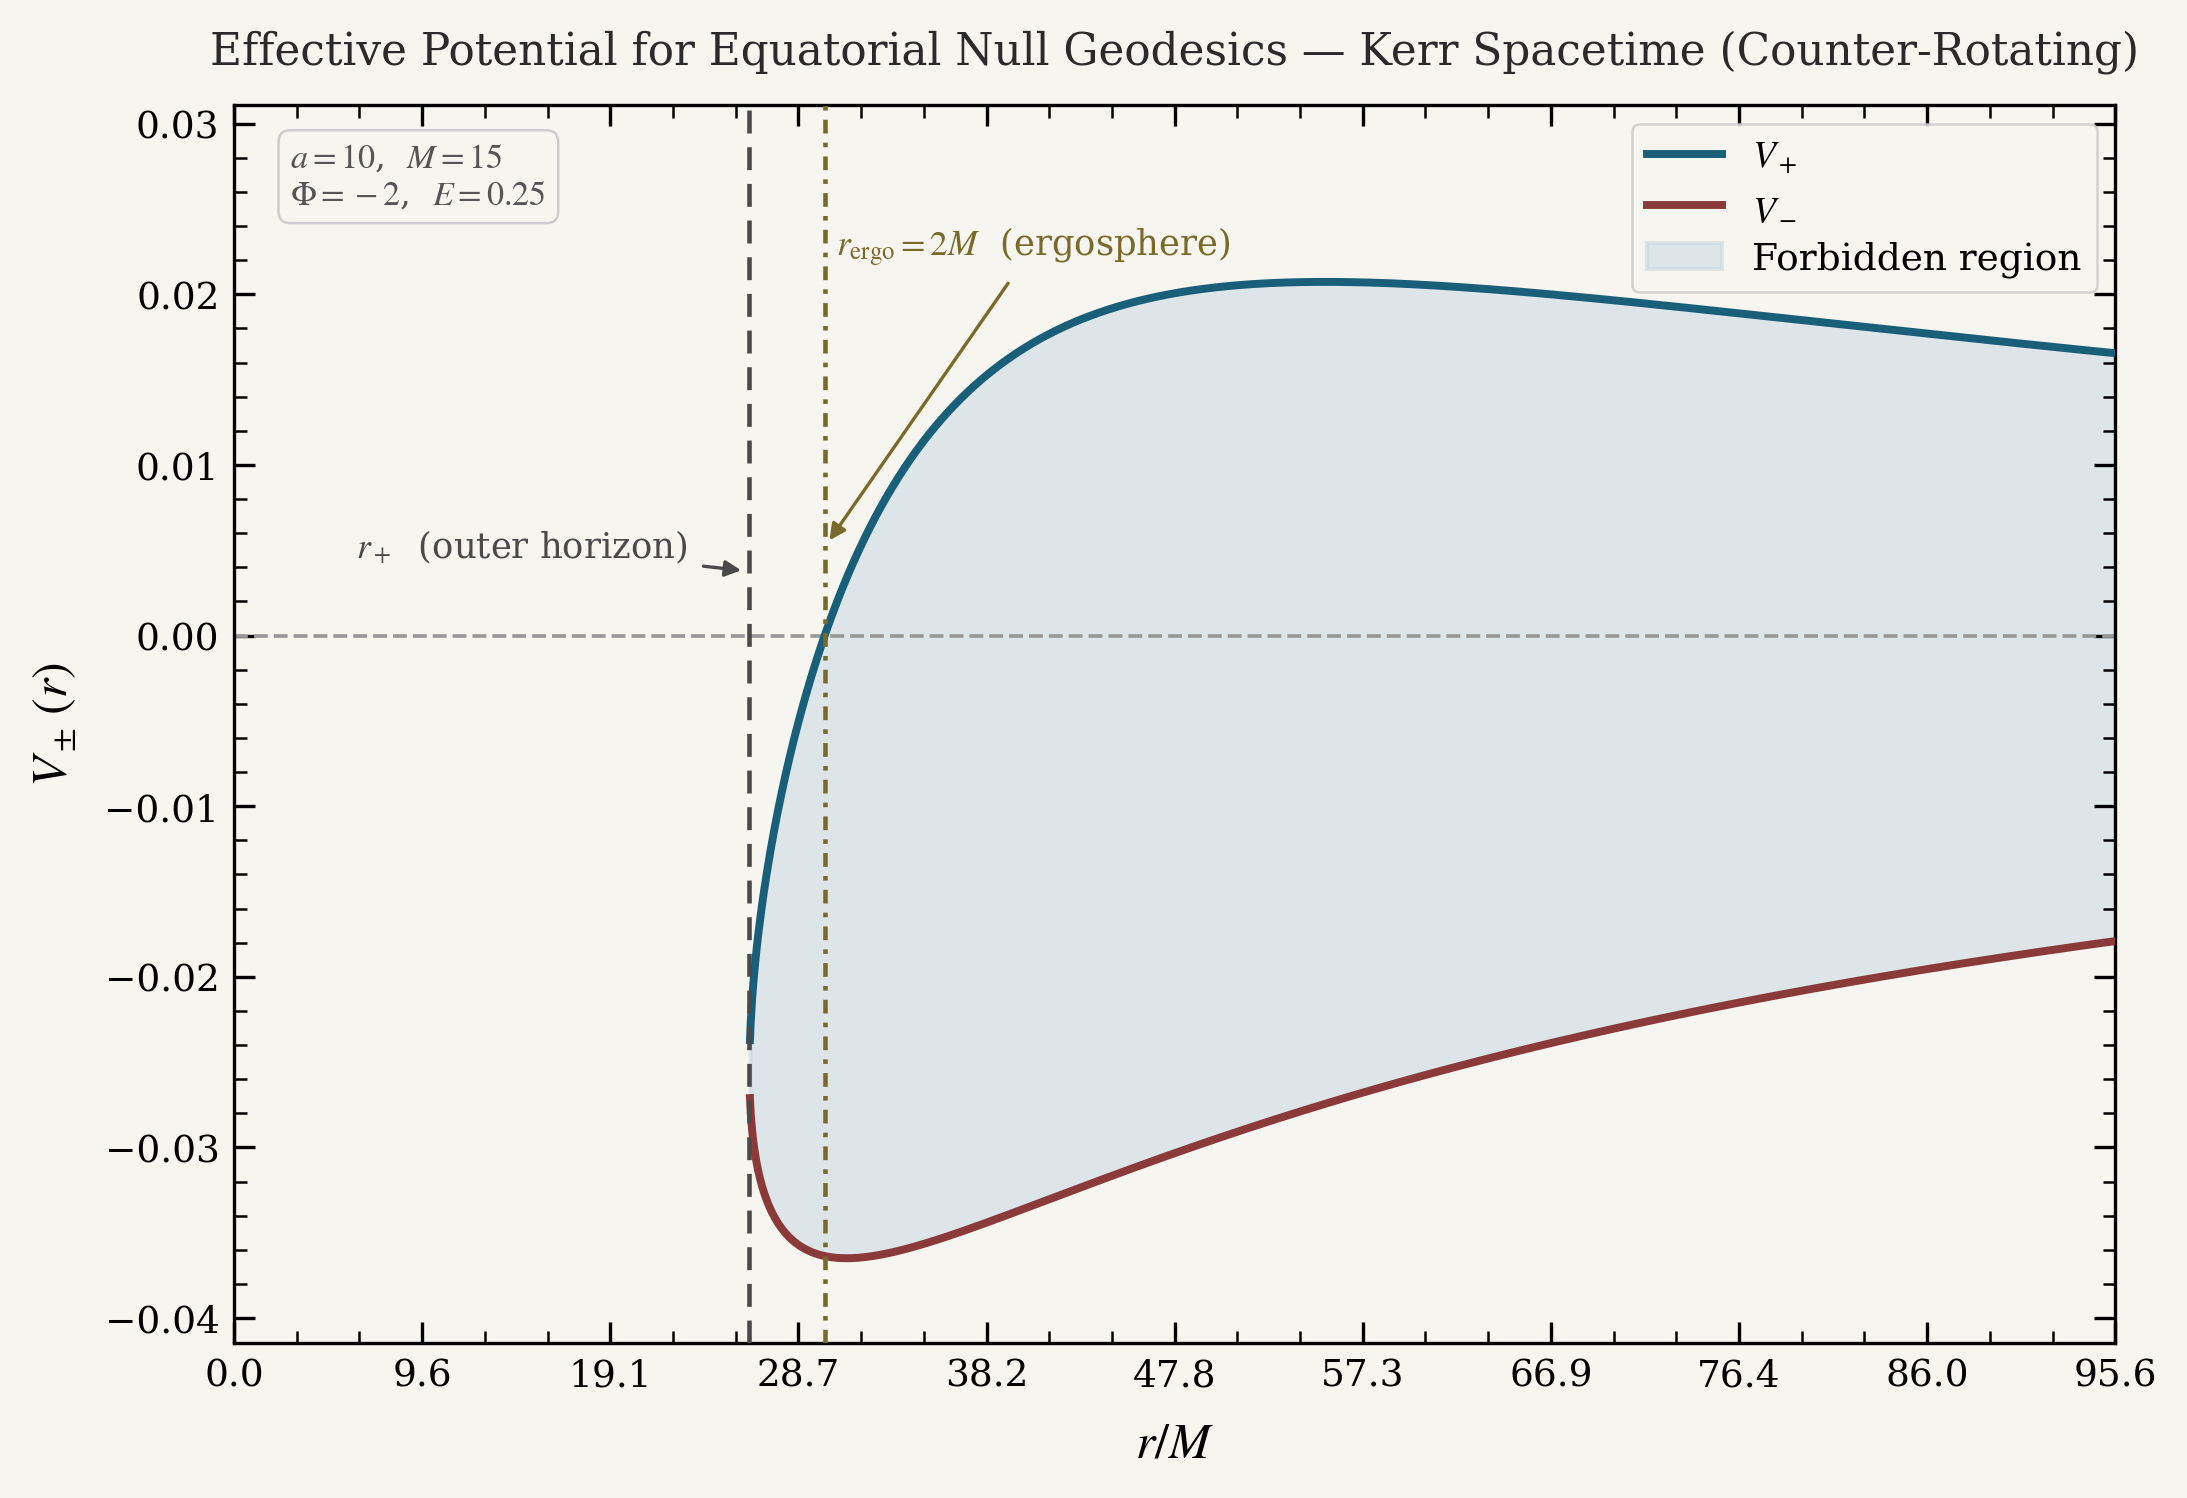
\includegraphics[width=0.83\textwidth]{figures/kerr_potential_counterrotating.png}
    \caption{Sketches of Effective Potential for Counter-Rotating Photons in Kerr Spacetime.}
    \label{fig:counter_potential_sketch}
\end{figure}

\begin{figure}[H]
    \centering
    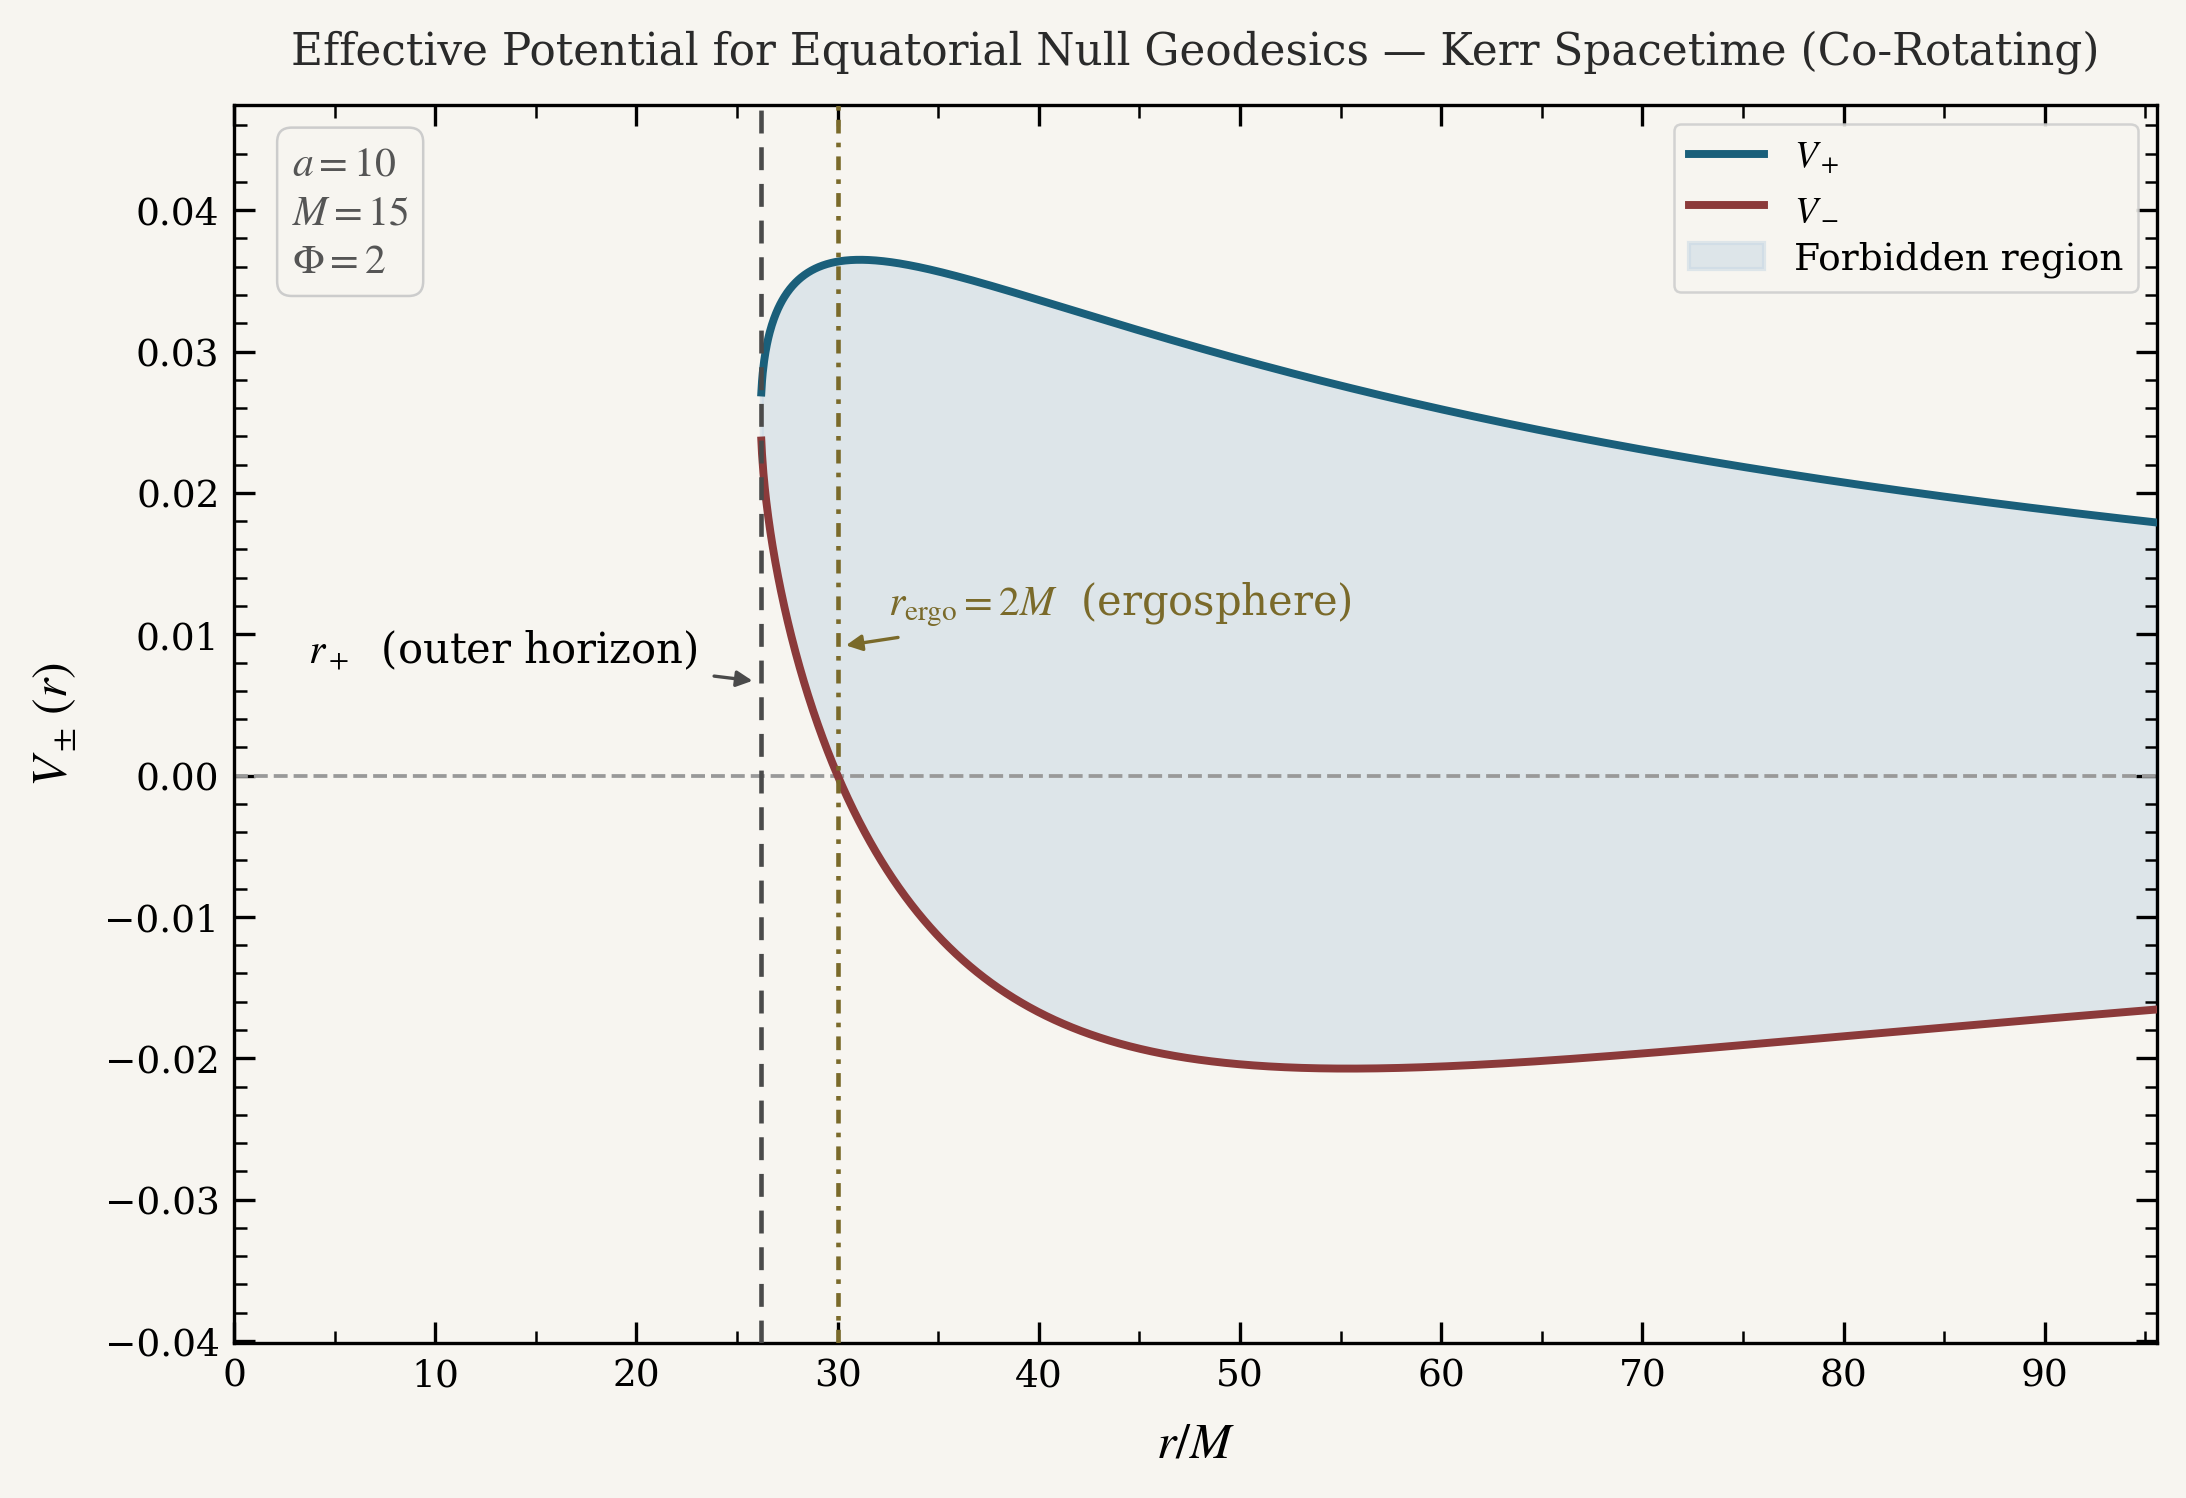
\includegraphics[width=0.83\textwidth]{figures/kerr_potential_corrotating.png}
    \caption{Sketches of Effective Potential for Co-Rotating Photons in Kerr Spacetime.}
    \label{fig:co_potential_sketch}
\end{figure}

One case during this motion is when the particle starts from far away with some finite energy and approaches the black hole. It will be able to cross the horizon if its energy is greater than the maximum of $V_+$. This is a case of photon capture.\smallskip

If it is less than the maximum of $V_+$ then it will have a turning point somewhere outside the horizon and will reverse its direction back to infinity. This is the case of deflection.\bigskip

The other case pertains to motion of co-rotating photons between the outer event horizon and the maximum of $V_+$. It is only allowed to exist in this region within the range of $V_+(r_+) < E < V_+(r_{max})$.\smallskip

The last case is that of counter-rotating photons between the ergosphere (where $V_+ = 0$) and the outer event horizon. Here, the energy of the particle can be negative and it can exist in the range of $V_+(r_+) < E < 0$. The existence of this "negative energy" is due to the fact that the time Killing vector becomes spacelike in the ergosphere and therefore, the energy of the particle as measured by an observer can be negative. This is the same concept used during the description of the Penrose process. \bigskip

We can also see that there are two unstable circular orbits present here - one prograde (co-rotating case) and one retrograde (counter-rotating case). These orbits are located at the maximum of $V_+$ and will be discussed in detail below in the section on spherical orbits. \bigskip

\begin{framed}
\textbf{Note:} Finally, we can expand this discussion to all non-spherical trajectories - including those that are timelike and lie outside the equatorial plane. Their qualitative nature also follows the same treatment. Although, in such cases, the energy ranges will get modified due to the presence of the non-zero $\kappa$ and $\theta$ terms in the geodesic equations. 
\end{framed}

\subsection*{Spherical Orbits}
Spherical orbits constitute those special cases where the radial coordinate remains constant throughout the motion of the particle. However, the particle is free to move in the $\theta$ and $\phi$ directions. 

The conditions for spherical orbits can be derived from the radial geodesic equation (\ref{eq:geodesic_equations}a). For a spherical orbit, the radial velocity and the radial acceleration must both be zero. This leads to the following conditions:

\[ R(r) =0, \qquad \dot{R}(r) =0 \]

There are, however, restrictions on the motion of the particle in the $\theta$ plane. $V(u)$ in the $\theta$ geodesic equation (\ref{eq:geodesic_equations}b) must also be non-negative for the particle to be able to move in the latitudinal direction. This gives us the following condition,

\[ V(u) \geq 0, \qquad |u| < 1\]

Therefore, we have to look for values of u for which the above conditions are satisfied - which is done by looking at the behavior of the roots of $V(u)$. The solutions of this equation allow for the latitude variable, $u$, to exist within a certain range. At the boundaries of this range, the particle will have a turning point in the $\theta$ direction and will reverse its motion.\smallskip 

Therefore, the motion in the $\theta$ direction is oscillatory between these two turning points.\medskip

Now it is time to analyze this periodic motion in the context of timelike and lightlike geodesics.

\subsubsection*{Lightlike Trajectories}
We can rewrite the $\theta$ geodesic equation (\ref{eq:geodesic_equations}b) for photons as follows,

\begin{equation} \label{eq:theta_geodesic_photon}
    (\frac{\Sigma}{E})^2 \dot{u}^2 = \mathcal{Q} - (\mathcal{Q} + \varPhi^2 -a^2)u^2 - a^2u^4
\end{equation}

where,

\[ \mathcal{Q} = \frac{Q}{E^2}, \qquad \varPhi = \frac{\Phi}{E} \]

This equation is quadratic in $w = u^2$ and gives us an idea about the roots of $V(u)$ depending on the sign of $\mathcal{Q}$.

According to the conditions outlined in the previous section, non-negative values of $w$ can only exist when $\mathcal{Q}\geq 0$ \cite{taoPhotonSpherical}. Therefore, we will consider only this case for the rest of our discussion. The positive roots for the above equation for non-negative $\mathcal{Q}$ are given by,

\begin{subequations}
\begin{align*}
    u_0^2 &= \frac{(a^2 - \mathcal{Q} - \varPhi^2) + \sqrt{(a^2 - \mathcal{Q} - \varPhi^2)^2 + 4a^2\mathcal{Q}}}{2a^2} & {\mathcal{Q}>0} \\
    u_0^2 &= 0 & {\mathcal{Q} = 0} \\
\end{align*}
\end{subequations}

\parHeading{$\mathcal{Q}>0$}: Here the particle reaches a maximum latitude of $u_0$ and then reverses its direction. The motion in the $\theta$ direction is oscillatory between $-u_0$ and $u_0$.\medskip

\parHeading{$\mathcal{Q}=0$}: This represents an unstable circular orbit where the particle starts in the equatorial plane with zero velocity in the $\theta$ direction and stays in the equatorial plane. These are the unstable circular orbits described above.

\begin{framed}
    \parHeading{Note:} If we set $u=0$ (equatorial plane) in the geodesic equation (\ref{eq:theta_geodesic_photon}) we get $r^2\dot{\theta} = \pm\sqrt\mathcal{Q}$ which is the condition for equatorial orbits. Therefore, physically, the Carter's constant can be interpreted as a measure of the angular speed of the photon while crossing the Black Hole's equator. 
\end{framed}

Now that we have deduced the motion in the $\theta$ direction, we can turn to the radial geodesic equation. Setting $R(r)$ and its derivative to zero, we can find the conditions for spherical photon orbits. These restrictions give us the expressions for $\mathcal{Q}$ and $\varPhi$ in terms of the radius of the orbit, $r$,

\begin{equation} \label{eq:phi_spherical_photon}
    \varPhi = -\frac{r^3 - 3Mr^2 + a^2r + a^2M}{a(r-M)}
\end{equation}

\begin{equation} \label{eq:Q_spherical_photon}
    \mathcal{Q} = -\frac{r^3(r^3 - 6Mr^2 + 9M^2r - 4a^2M)}{a^2(r-M)^2}
\end{equation}

The azimuthal direction requires a more careful analysis. The $\phi$ geodesic equation can be rewritten in terms of $w$ using (\ref{eq:geodesic_equations}c) and (\ref{eq:geodesic_equations}d) as follows,

\begin{equation}
    \frac{d\phi}{dw} = \frac{1}{Y(w)}\Big[\frac{\varPhi}{2(1-w)} + \frac{2Mra - a^2\phi}{2\Delta}\Big]
\end{equation}
where
\[ Y^2(w) = \mathcal{Q}w - (\mathcal{Q} + \varPhi^2 -a^2)w^2 - a^2w^3 \]

Integrating these expressions can provide us with analytical values of $\Delta\phi$ for one period of oscillation in the $\theta$ direction. 

The velocity in the $\phi$ direction is not always prograde or retrograde. From (\ref{eq:geodesic_equations}c), we can see that $\dot{\phi}$ changes sign when $u$ hits the following value,

\begin{equation}
    u_1^2 = \frac{r^2(3M-r)}{a^2(r+M)}
\end{equation}

Of course, this is only relevant when the photon is actually able to reach this point or when $u_1 < u_0$. 

\begin{framed}
Therefore, the velocity in the $\phi$ direction may reverse at certain points. But, overall, the orbit can be described as retrograde or prograde depending on the sign of $\varPhi$. As it is representative of the total displacement in the $\phi$ direction per latitudinal oscillation. 
\end{framed}

\begin{figure}[H]
    \centering
    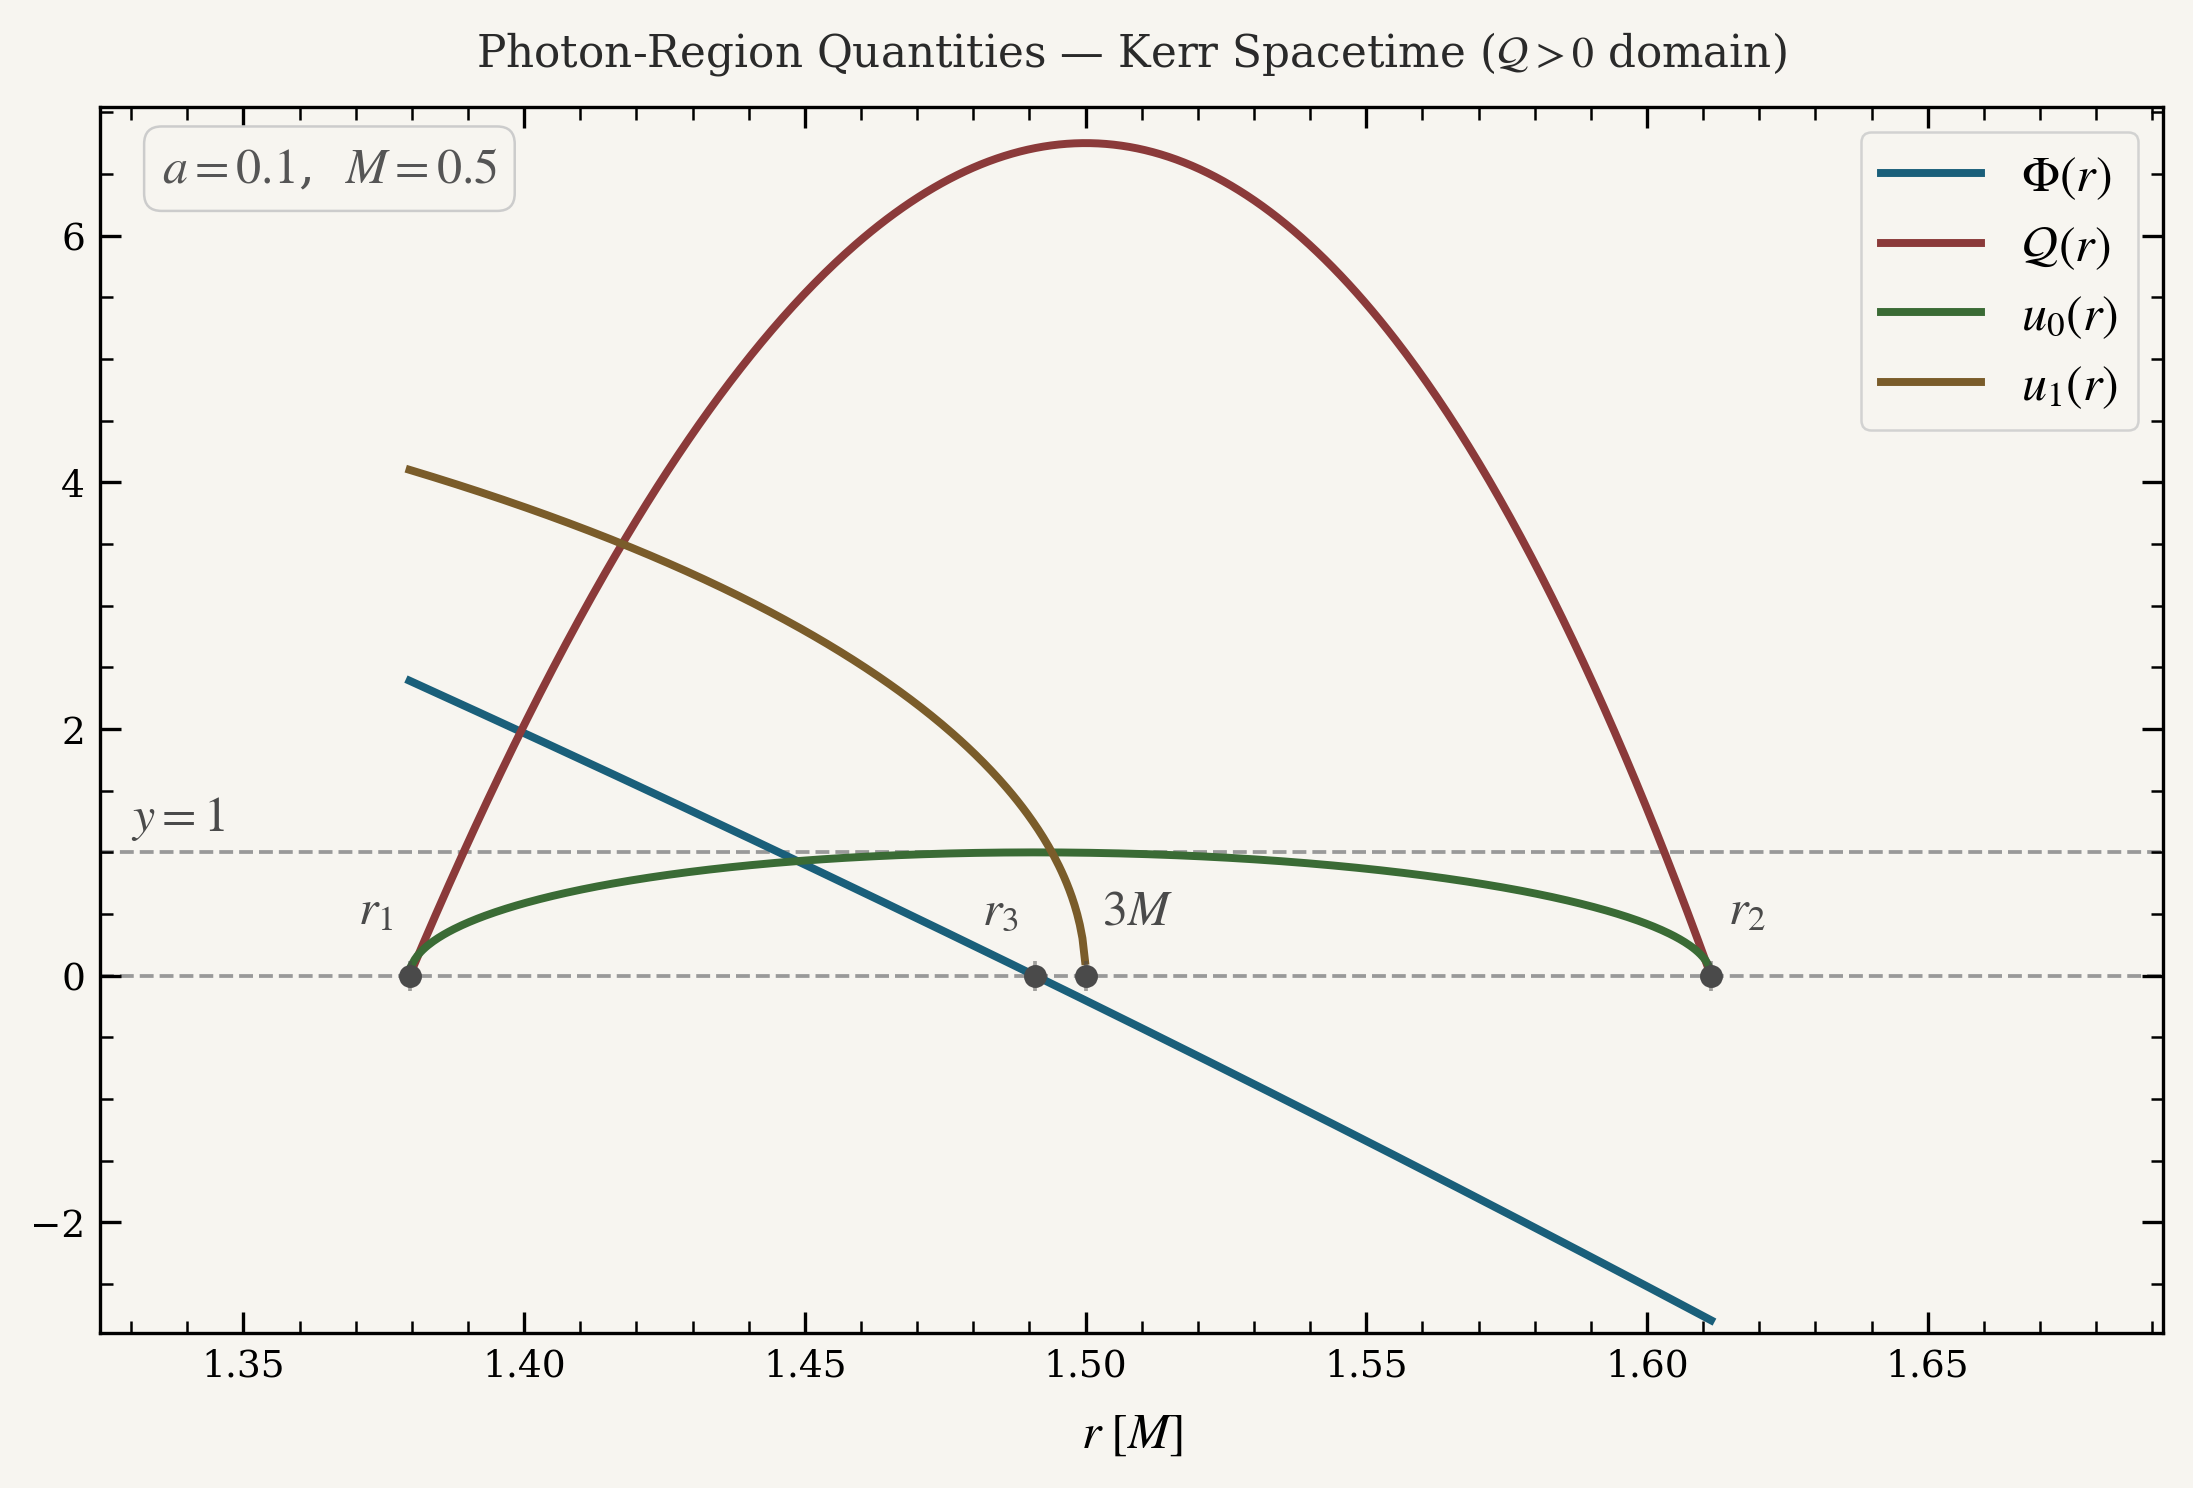
\includegraphics[width=0.9\textwidth]{figures/kerr_photon.png}
    \caption{Variation of $\varPhi, \mathcal{Q}, u_0$ and $u_1$ with changing radius of the orbit. Note that these values are only considered in the region between the two circular orbits as discussed.}
    \label{fig:parameter_values_photon}
\end{figure}

In the plot (Figure \ref{fig:parameter_values_photon}), we see that $\mathcal{Q}$ is positive in the range between two specific radii. These two radii represent the two unstable circular orbits in the equatorial plane - one is the prograde and the other is the retrograde one. The radii of these orbits are,

\begin{subequations}
    \begin{align}
        r_1 &= 2M\Big\{1 + \cos\Big[\frac{2}{3}\arccos\Big(-\frac{|a|}{M}\Big)\Big]\Big\} \\
        r_2 &= 2M\Big\{1 + \cos\Big[\frac{2}{3}\arccos\Big(\frac{|a|}{M}\Big)\Big]\Big\}
    \end{align}
\end{subequations}

We also see that the increase in the maximum latitude of the photon is associated with a decrease in the angular momentum of the photon in the $\phi$ direction. This relates to the conservation of total angular momentum for the photon. $\varPhi$ hits zero at the same point when $u_0$ hits its maximum value of $1$ where it can reach the poles. The spherical orbits shift from being prograde to retrograde at the radius where $\varPhi$ changes sign, given by,

\begin{equation}
    r_3 = M + 2\sqrt{M^2 - \frac{a^2}{3}}\cos\Big[\frac{1}{3}\arccos\frac{M(M^2-a^2)}{(M^2 - \frac{a^2}{3})^{\frac{3}{2}}}\Big]
\end{equation}

\parHeading{Note:} A word about $\Delta \phi$ - it has a discontinuity at $r_3$. This occurs because the photon reaches its maximum latitude at the poles during this orbit. A small perturbation on either side would add or subtract a full $2\pi$ to the total displacement in the $\phi$ direction. In one case it would swing around the poles - adding a $2\pi$ - and in the other it would miss the poles and end up with a retrograde displacement - subtracting a $2\pi$.

\subsubsection*{Timelike Trajectories}
The situation is more complicated in the case of timelike trajectories as the non-zero $\mu$ does not allow us to effectively factor out the energy as a normalization factor - as we did in the case of photons. Here the roots of $V(u)$ are as follows for the case of $\mu = 1$,

\begin{equation} \label{eq:w_roots}
   w_{1,2} = u_{1,2}^2 = \frac{1}{2a^2(1-E^2)}\Big[a^2(1-E^2) + \Phi^2 + Q \mp \sqrt{(a^2(1-E^2) + \Phi^2 + Q)^2 - 4a^2Q(1-E^2)}\Big]
\end{equation}

Similarly, the radial geodesic equation cannot be parametrized in terms of $\mathcal{Q}$ and $\varPhi$ and will be better off being parametrized by $r$ and $Q$. Therefore, using the velocity and acceleration conditions for spherical orbits, the energy and angular momentum of the photon can be written as,

\begin{equation} \label{eq:energy_spherical_timelike}
    E_{a,b} = \frac{r^3(r-2M) - a(aQ \mp \sqrt{\Upsilon})}{r^2\sqrt{r^3(r-3M) -2a(aQ \mp \sqrt{\Upsilon})}}
\end{equation}

\begin{equation} \label{eq:angular_momentum_spherical_timelike}
    \Phi_{a,b} = -\frac{2Mar^3 + (r^2+a^2)(aQ \mp \sqrt{\Upsilon})}{r^2\sqrt{r^3(r-3M) -2a(aQ \mp \sqrt{\Upsilon})}}
\end{equation}

where,

\begin{equation}
    \Upsilon = Mr^5 - Q(r-3M)r^3 + a^2Q^2
\end{equation}

There are actually four branches of the solutions here. The above $(a,b)$ branches are those with positive energies and the other two - $(c,d)$ - are those with negative energies. Negative energies can exist in the ergosphere of the Black Hole. We will analyze the positive energy solutions in this paper and the negative cases can be trivially obtained by $E_{c,d} = -E_{a,b}$.

Using the restrictions on the various square roots and the non-negative nature of both $R(r)$ and $V(u)$, we can define the parameter space (values of $r$ and $Q$) for which spherical orbits can exist. 

Before we produce the parameter space, we will discuss the nature of these orbits. Namely, the orbits will be classified on the basis of the following criteria:

\begin{itemize}
    \item \parHeading{Prograde vs Retrograde}: Prograde orbits are those that are co-rotating with the black hole, while retrograde orbits are those that are counter-rotating. The sign of $\Phi$ can be used to determine whether the orbit is prograde or retrograde.
    \item \parHeading{Stable vs Unstable}: Stable orbits are those that are stable under small perturbations, while unstable orbits are those that are not. The stability of an orbit can be determined by analyzing the second derivative of $R(r)$ (\ref{eq:radial_potential}) at the radius of the orbit.
    \item \parHeading{Bound vs Unbound}: Bound orbits are those that permit values in a finite range of radii outside the event horizon, while unbound orbits extend till infinity. The criteria to distinguish them is given by the behavior of $R(r)$ at infinity. At large radii, only the leading coefficient of $(E^2 - \mu^2)$ plays a role in determining the sign of $R(r)$. If $R(r)$ is positive until infinity, then the orbit is unbound as motion even at diverging radii is allowed. If $R(r)$ starts to tend to negative values at $r$ increases then it is a bound orbit and the particle cannot escape to infinity. These are respectively the cases of $E^2 > 1$ and $E^2 < 1$ for timelike trajectories - with $E^2 = 1$ being the critical case of marginally bound orbits.
\end{itemize}

All three of these criteria can be determined by looking at the value of $Q$. Namely, boundaries of $Q$ exist for each radius $r$ that separate the parameter space into different regions corresponding to different orbits. The marginal values of $Q$ that define these boundaries are given by $Q_{mb}, Q_{ms}, Q_o$ for the bound, stable and prograde/retrograde boundaries respectively. These are given by the following expressions,

\begin{subequations}
    \begin{align}
        Q_{ms} = -\frac{Mr^{5/2}[(\sqrt{\Delta} - 2\sqrt{Mr})^2 - 4a^2]}{4a^2(r^{3/2} - M\sqrt{r}- \sqrt{M \Delta})} \\
        Q_{mb} = -\frac{Mr^2[r(\sqrt{r} - \sqrt{2M})^2 - 4a^2]}{a^2(\sqrt{r} - \sqrt{M})^2} \\
        Q_o = \frac{Mr^2(\Delta^2 + 4Mr^2(r-M))}{(r^2+a^2)(r\Delta - M(r^2-a^2))}
    \end{align}
\end{subequations}

Keep in mind that the criterion related to angular momentum and $Q_o$ is only relevant past a certain radius, as $Q_o$ is negative for radii smaller than a certain $r_o$. This radius is given by the following expression and the orbits are all prograde for $r<r_o$ irrespective of the value of $Q$ in this range.

\[ r_o = M + 2\sqrt{\frac{3M^2-a^2}{3}}\cos\Big(\frac{1}{3}\arccos\Big(\frac{3M(M^2-a^2)}{3M^2 - a^2}\sqrt{\frac{3}{3M^2-a^2}}\Big)\Big) \]\bigskip

\parHeading{Summary of Timelike Spherical Orbits:}
The various regimes of solutions can be divided using the two photon circular orbits of radii $r_1$ and $r_2$,
\begin{itemize}
    \item \parHeading{$r = r_1, a=M$}: For the extremal Kerr black hole, there is a stable circular prograde orbit at the horizon. This is a special case and is called a horizon-skimming orbit. For more information about this case, see \cite{taoTimelikeSpherical}.
    \item \parHeading{$r_1 \leq r < r_2$}: There is always a $Q=0$ solution that corresponds to a stable circular prograde orbit. The particle starts its latitudinal oscillations (much like the photons) when $Q$ is increased. In this range, only the first class ($a$) of solutions of energy (\ref{eq:energy_spherical_timelike}) and angular momentum (\ref{eq:angular_momentum_spherical_timelike}) are possible and $Q$ can take any positive value. As $Q$ is increased, the orbits become to begin to move towards the unstable and unbound range. 
    \item \parHeading{$r = r_2$}: Here, there are restrictions on the value of $Q$ and it can only follow the range $ 0 \leq Q < 32M^2$. As $Q$ moves towards the upper limit, this orbit reduces to the unstable circular retrograde orbit at this radius. Only the $a$ branch of the solutions exist here.
    \item \parHeading{$r>r_2$}: The range of $Q$ is equal to $0 \leq Q < Q_1$ where the upper limit has the following expression,
    \[Q_1 = \frac{r^2}{2a^2}(r(r-3M)\mp \sqrt{r\Xi})\]
    where,
    \[\Xi = r^3 - 6Mr^2 + 9M^2r - 4Ma^2\]
    \begin{framed}
    The $32M^2$ upper-limit in the previous case is the same that will be derived from this expression when $r=r_2$.
    \end{framed}
    However, now both branches $(a,b)$ are feasible with different parameter spaces. These two solutions converge at the the upper limit of $Q=Q_1$ and all orbits in the second branch are retrograde. 
\end{itemize}

We represent the parameter space within the range $r_1 \leq r < r_2$ in Figure \ref{fig:parameter_values_timelike}.
\begin{figure}[H]
    \centering
    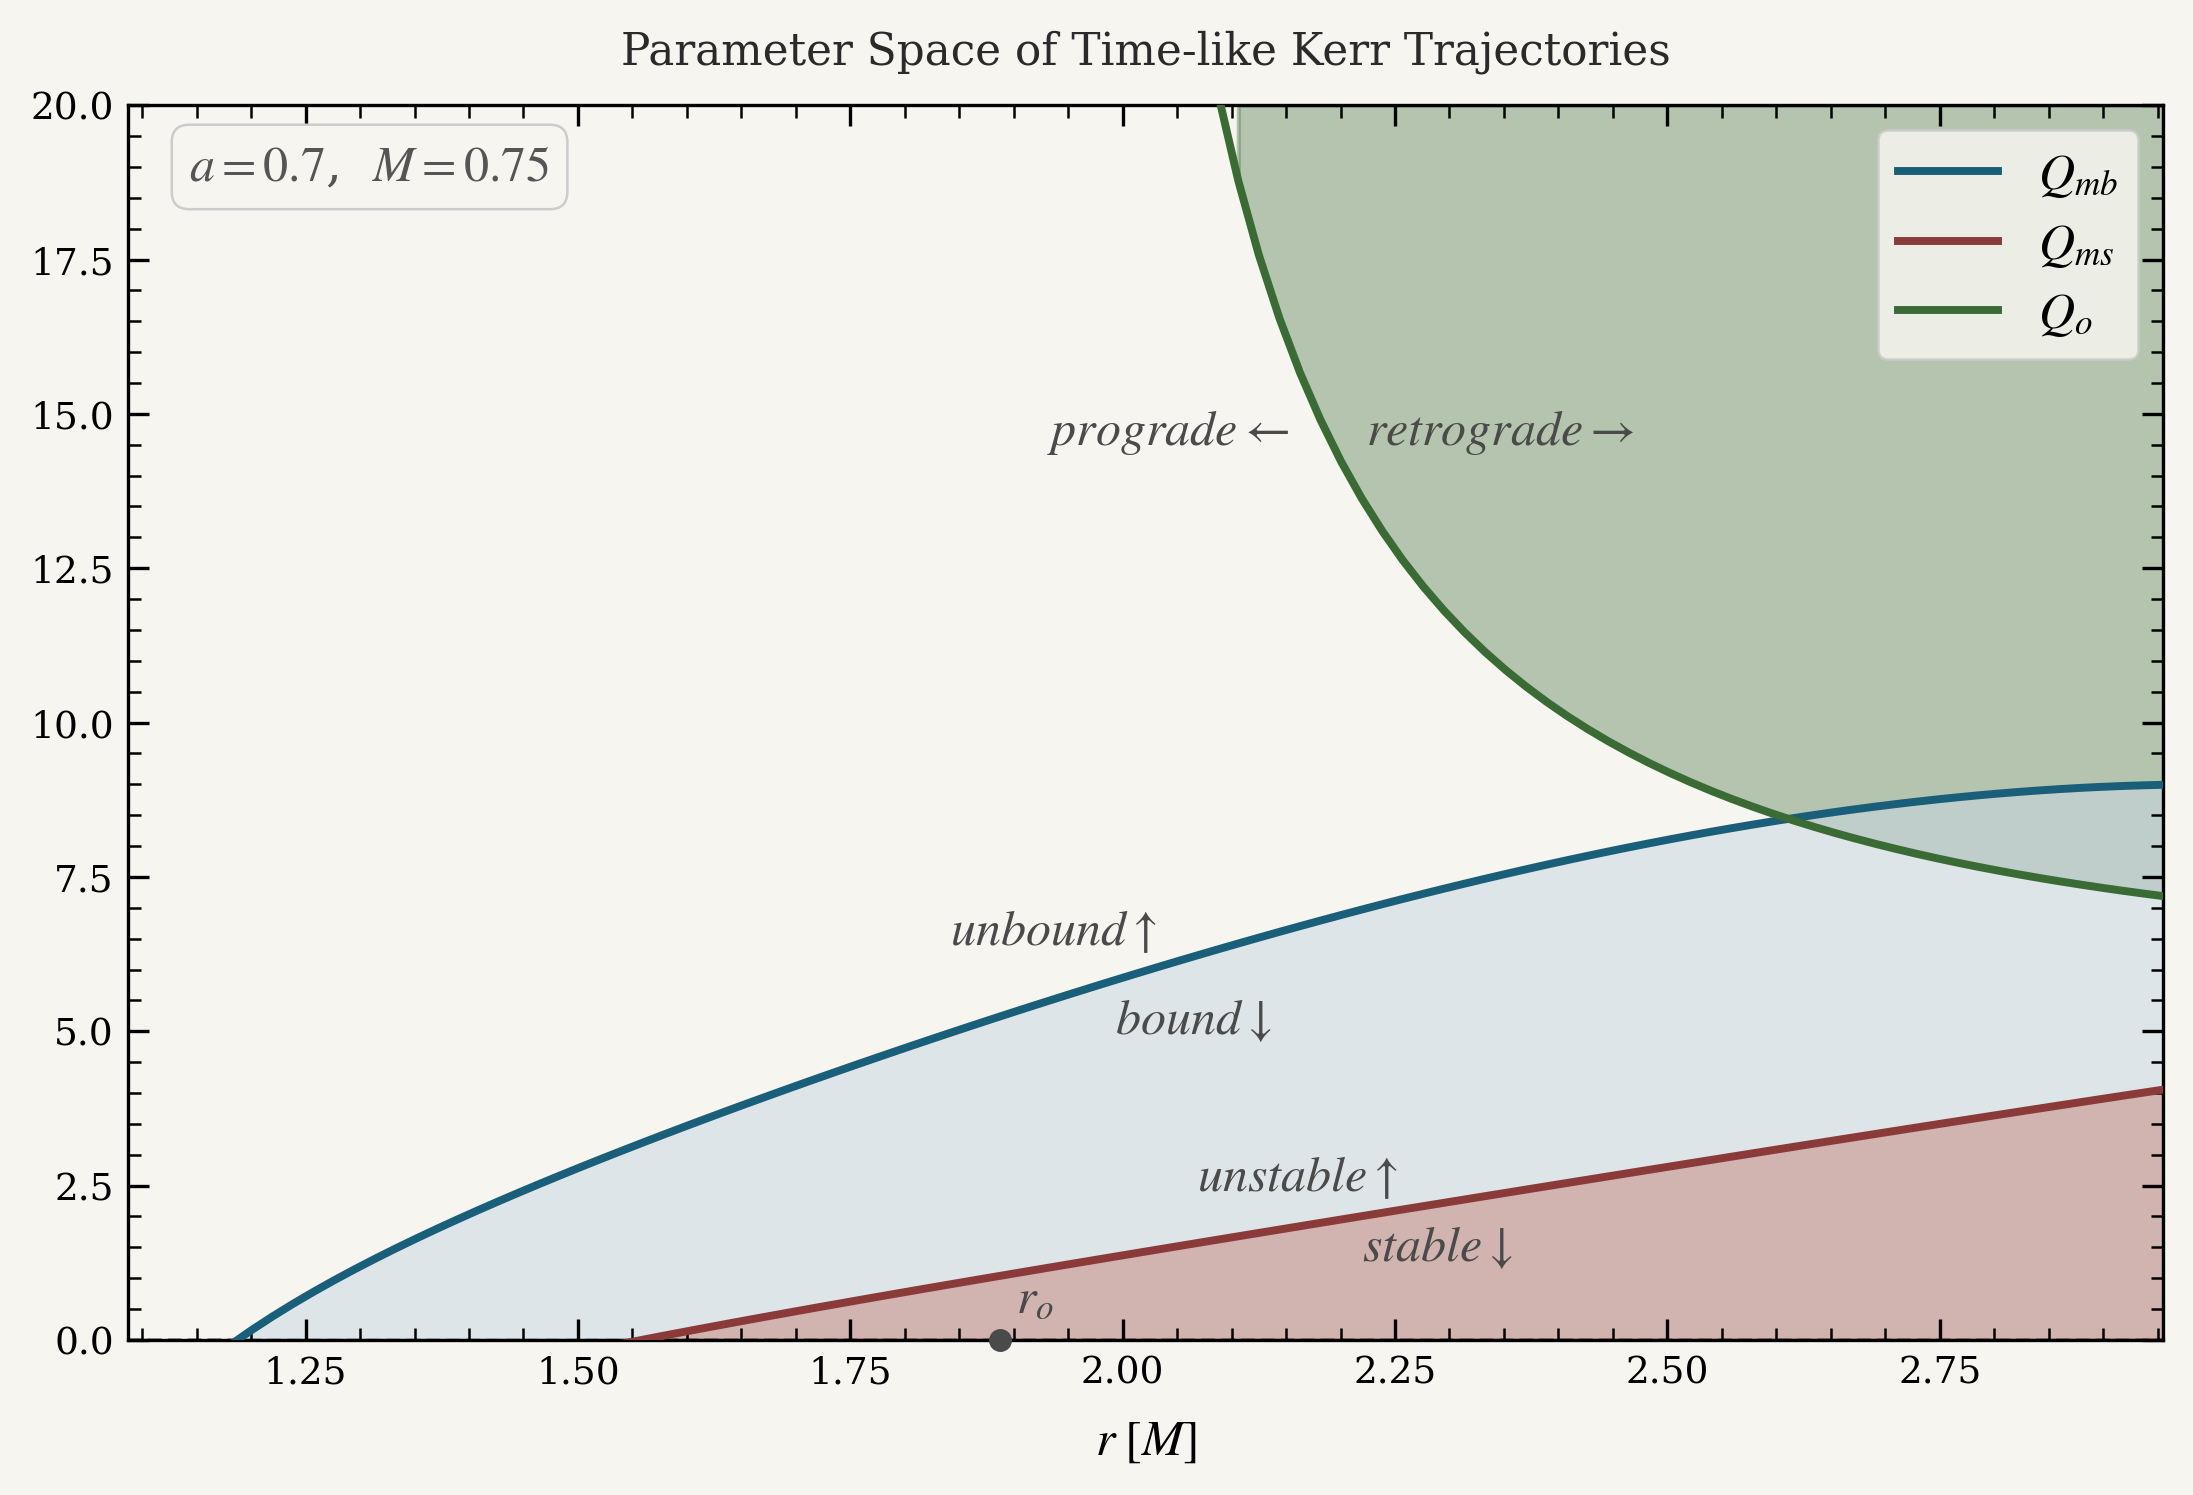
\includegraphics[width=0.9\textwidth]{figures/kerr_timelike_parameter_space.png}
    \caption{Parameter Space of timelike trajectories for a non-extremal Kerr Black Hole. Here, the boundaries for each criterion are presented and the radii range from $r_1 \leq r < r_2$.}
    \label{fig:parameter_values_timelike}
\end{figure}

Finally, we end our discussion with certain analytical solutions of the geodesical equation that can be found using Mino's Method \cite{taoTimelikeSpherical}. 

We will not go into the details of the derivation but the basis is the shift from using proper time as a parameter to, $\lambda$ which is given by,

\[ \Sigma \frac{x^\mu}{d\tau} = \frac{dx^\mu}{d\lambda}\]

and called Mino's parameter.\medskip

Here, we can write the geodesic equation in the $\theta$ direction as follows,

\begin{equation}
    \frac{dw}{d\lambda} = 2Y(w)
\end{equation}

where,

\[ Y^2(w) = a^2(1-E^2)w(w-w_1)(w-w_2) \]

where $w_{1,2}$ are the given by (\ref{eq:w_roots}).\medskip

Now, we integrate the equation - starting from the equator- to get $\lambda$ as a function of $w$, which can then be inverted.

\begin{equation}
    \lambda(w) = \int_0^{w} \frac{dw}{2Y(w)} = \frac{1}{a\sqrt{(1-E^2)w_2}F(\psi,k)}
\end{equation}
where,
\[ \psi = \arcsin\sqrt{\frac{w}{w_1}}, \quad k = \sqrt{\frac{w_1}{w_2}} \]
Here, $F(\psi,k)$ is the incomplete elliptic integral of the first kind. 

Inverting this, we get the following expression for $\psi$,

\begin{equation}
    \psi = \operatorname{am}(a\sqrt{(1-E^2)w_2}\lambda, k)
\end{equation}

A full oscillation continues from $\lambda = 0$ to $4\lambda_0$ where,

\[ \lambda_0 = \frac{K(k)}{a\sqrt{(1-E^2)w_2}} \]

Similarly, the $\phi$ and $t$ coordinates can also be expressed in terms of $w$ by integrating the geodesic equation (\ref{eq:geodesic_equations}). We get,

\begin{subequations}
    \begin{align}
    \phi(\lambda) = \frac{\Phi}{a\sqrt{(1-E^2)w_2}}\Pi(\psi, w_1, k) + (2MrE - a\Phi)\frac{a}{\Delta} \\
    t(\lambda) = -\frac{aE}{a\sqrt{(1-E^2)w_2}}\Big[ (1-w_2)F(\psi,k) + w_2E(\psi,k) \Big] + \frac{1}{\Delta}\Big[ E(r^2 + a^2)^2 - 2Mra\Phi \Big]\lambda
    \end{align}
\end{subequations}

Where $E(\psi,k)$ and $\Pi(\psi, w_1, k)$ are the incomplete elliptic integral of the second kind and third kind. While, $K(k)$ is the complete elliptic integral of the first kind.

These integrals will only be consistent with the periodicity of the $\theta$ and $\phi$ motion if the following conditions are satisfied,

\begin{subequations}
    \begin{align}
        F(-\psi, k) = - F(\psi, k) && F(\psi+ \pi, k) = F(\psi, k) + 2K(k)\\
        \Pi(-\psi, w_1, k) = - \Pi(\psi, w_1, k) && \Pi(\psi + \pi, w_1, k) = \Pi(\psi, w_1, k) + 2\Pi(w_1, k)\\
        E(-\psi, k) = - E(\psi, k) && E(\psi + \pi, k) = E(\psi, k) + 2E(k)
    \end{align}
\end{subequations}

Keep in mind that this solution is valid only for bound orbits or $E^2<1$. For unbound orbits, the solution changes as follows,

\begin{subequations}
    \begin{align}
        k &= \sqrt{\frac{w_1}{w_1 - w_2}}, \qquad k \in (0,1) \\
        \psi &= \arcsin\sqrt{\frac{w(w_1 - w_2)}{w_1(w-w_2)}} = \operatorname{am}(a\sqrt{(E^2-1)(w_1-w_2)}\,\lambda,\, k)
    \end{align}
\end{subequations}

\begin{subequations}
    \begin{align}
        \phi(\lambda) &= \frac{\Phi}{a(1-w_2)\sqrt{(E^2-1)(w_1-w_2)}}\Big[F(\psi, k) - w_2\,\Pi(\psi,\, k^2(1-w_2),\, k)\Big]
        + \frac{a}{\Delta}(2MrE - a\Phi)\,\lambda \\
        t(\lambda) &= -\frac{aE}{\sqrt{(E^2-1)(w_1-w_2)}}\Big[ (1-w_2)F(\psi,k) + w_2\,\Pi\!\left(\psi,\, k^2,\, k\right)\Big]
        + \frac{1}{\Delta}\Big[ E(r^2+a^2)^2 - 2Mra\Phi \Big]\lambda
    \end{align}
\end{subequations}

\begin{equation}
    \lambda_0 = \frac{K(k)}{a\sqrt{(E^2-1)(w_1-w_2)}}
\end{equation}


An example for a selected orbit is shown in the figure below for an extremal black hole. The radius is selected as $r=1.2M$ and the Carter's constant is selected as $Q = 0.5M^2$. We can see that the particle reaches the maximum latitude and then drops - consistent with our analysis. The particle also has a prograde motion in the $\phi$ direction as $\Phi$ is positive for this case. The numerical values of the maximum latitude, energy and angular momentum also agree with \cite{taoTimelikeSpherical} for this case. 

\begin{figure}[H]
    \centering
    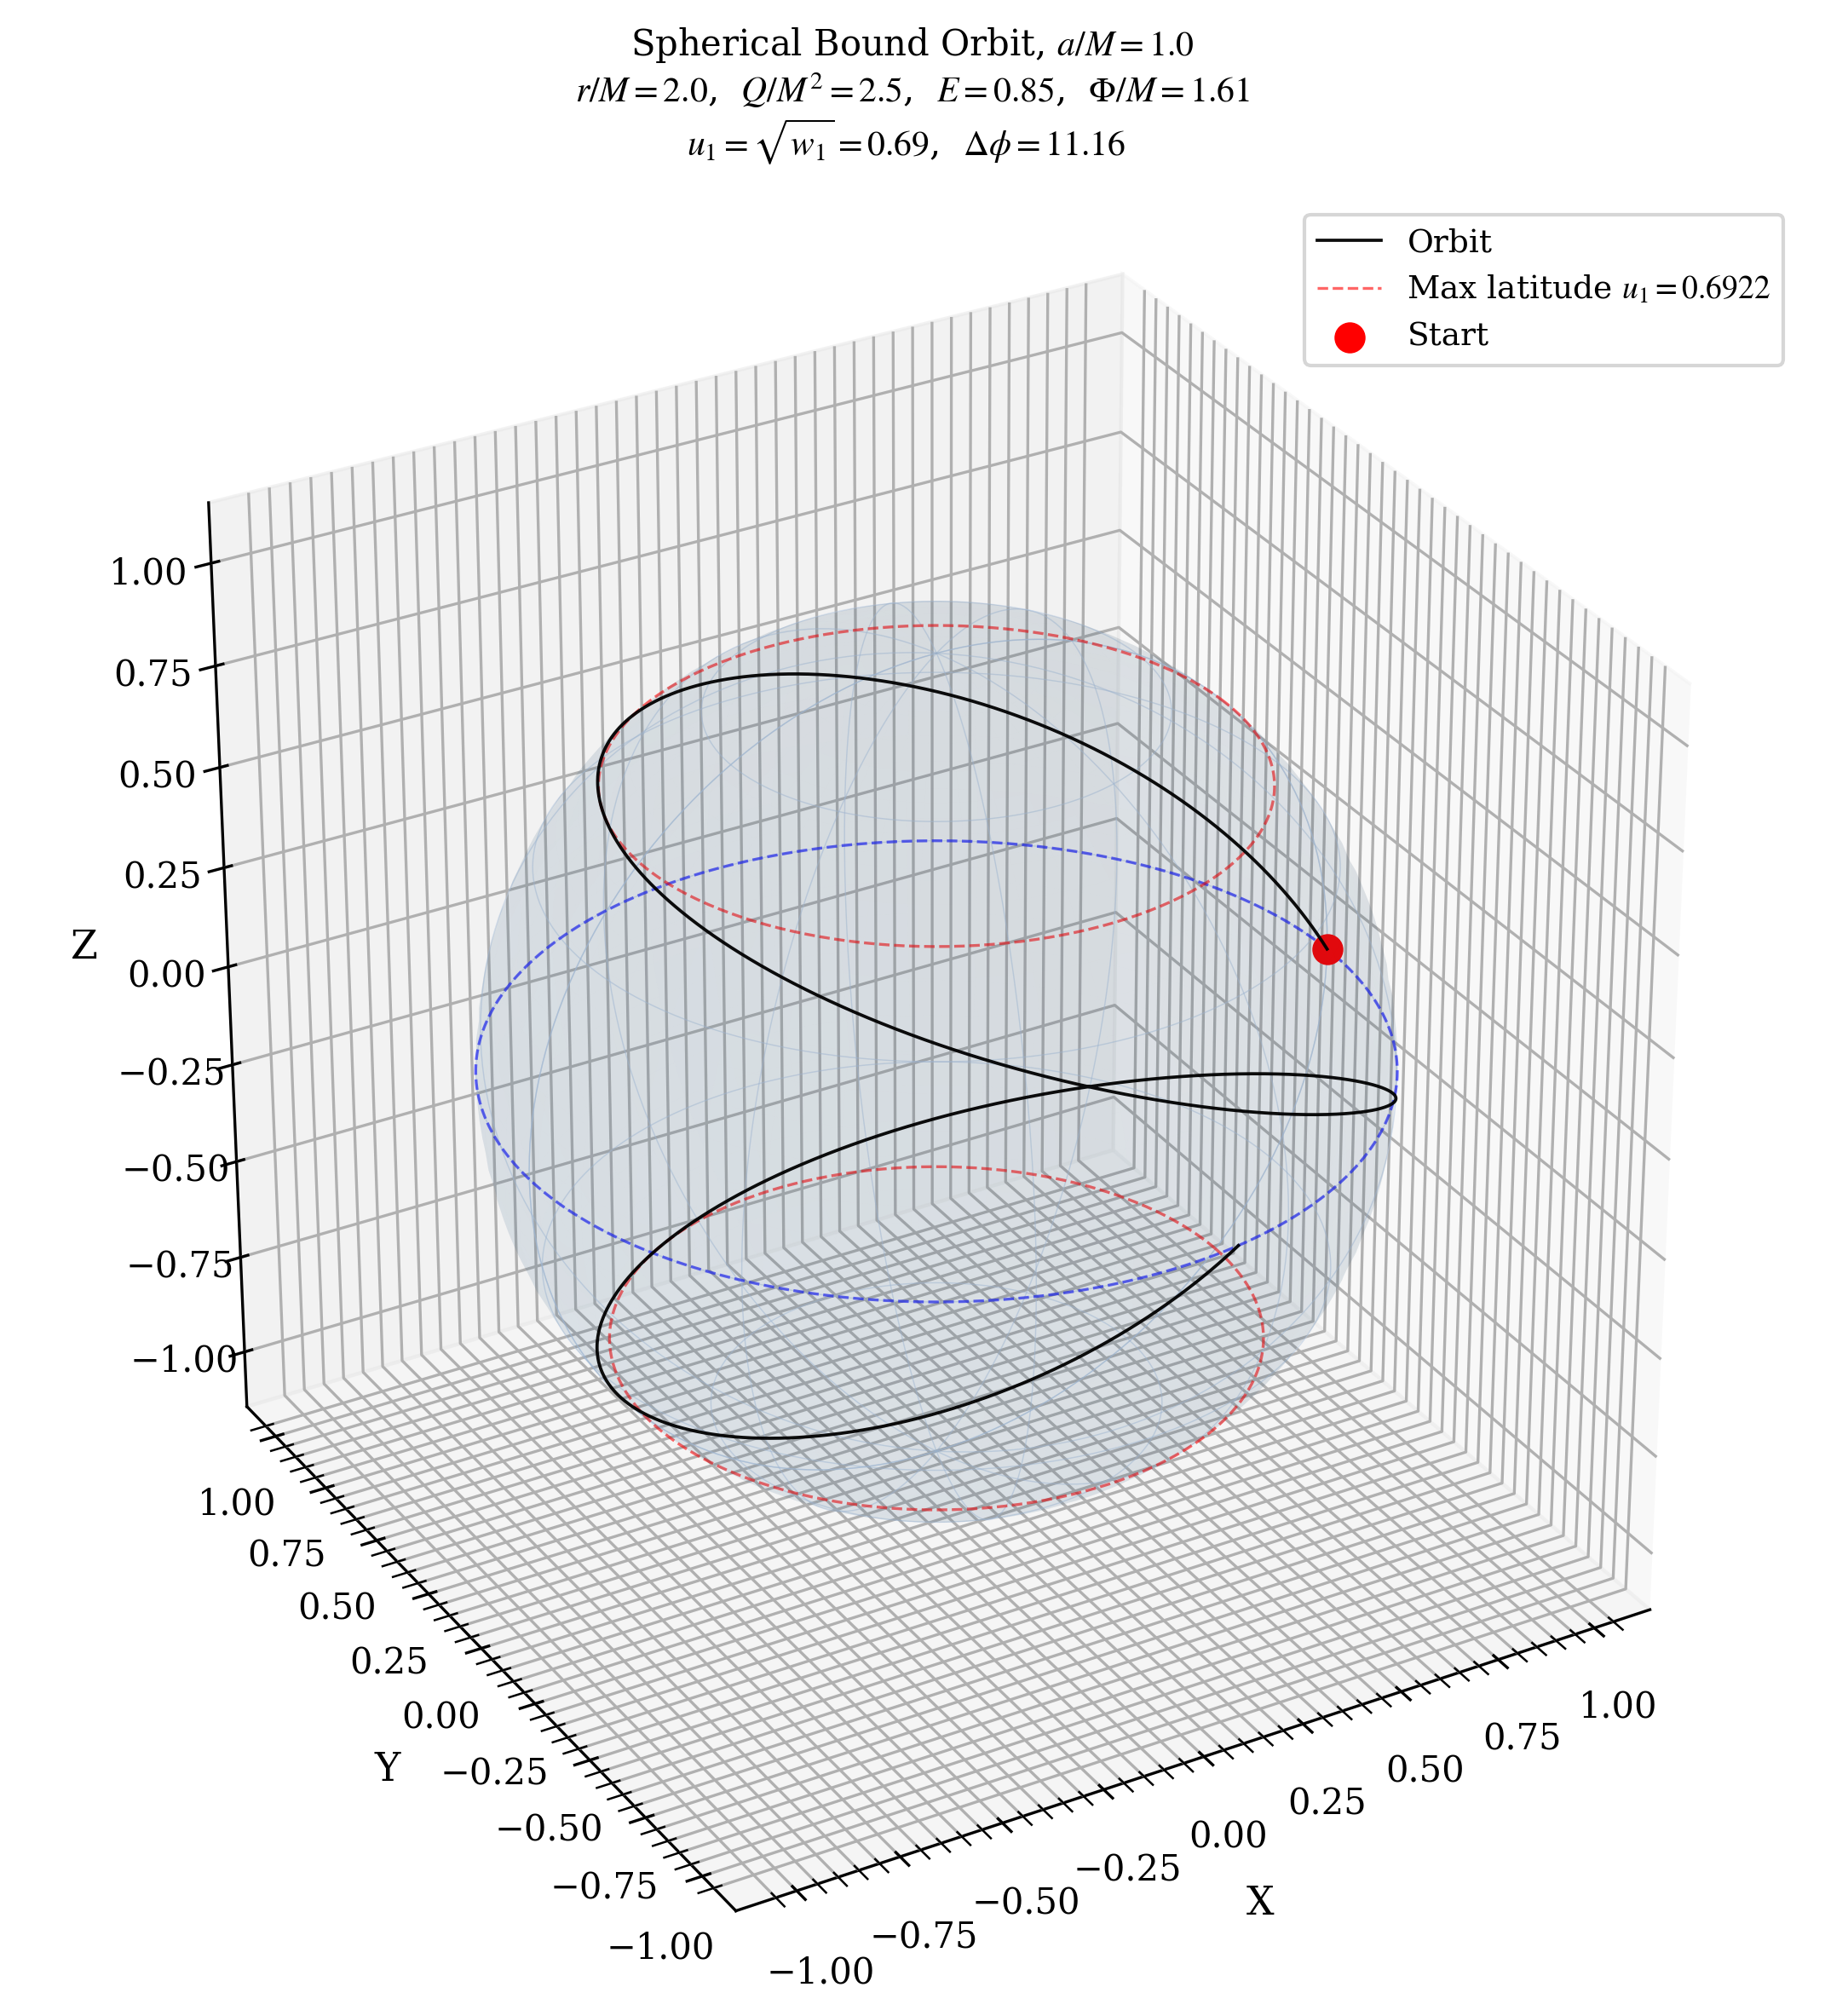
\includegraphics[width=0.8\textwidth]{figures/kerr_timelike_orbit.png}
    \label{fig:timelike_orbit}
    \caption{Example of a Timelike Spherical Orbit for an Extremal Kerr Black Hole.}
\end{figure}

\printbibliography

\end{document}
